\documentclass[a4paper, 11pt]{article}

\usepackage{cite}
\usepackage[english]{babel}
\usepackage[utf8]{inputenc}
% \usepackage[IL2]{fontenc}  
% \usepackage{amsmath,amsthm} 
% \usepackage{amsfonts}
\usepackage{amsmath, amsthm, amssymb} %units, dsfont

\usepackage[fixlanguage]{babelbib}
\selectbiblanguage{english}

\usepackage[pdfauthor={Jan Legersk\'y},
            pdfproducer={Jan Legersk\'y},
            pdfcreator={pdflatex},
            pdfencoding=unicode]{hyperref}
           
\usepackage{enumerate}
\usepackage[pdftex]{graphicx,color}

\usepackage{pgf,tikz}
\usepackage{mathrsfs}
\usetikzlibrary{arrows}

%\usepackage{comment}
%\excludecomment{proof}

\newcommand{\komentar}[1]{\textcolor{red}{#1} \newline}

\newcommand{\trcomp}{$\triangle$-component}
\newcommand{\trcomps}{$\triangle$-components}
\newcommand{\cv}[1]{c_v^{(#1)}}
\newcommand{\RR}{\mathbb{R}}

\DeclareMathOperator{\lcodim}{lcodim}
\DeclareMathOperator{\rank}{rank}

\newtheorem{thm}{Theorem}[section]
\newtheorem{lem}[thm]{Lemma}
\newtheorem{cor}[thm]{Corollary}
\newtheorem*{rem}{Remark}

\theoremstyle{definition}
\newtheorem{defn}{Definition}[section]
\newtheorem{exmp}{Example}[section]
\newtheorem{conj}{Conjecture}

\begin{document}
\begin{defn}
If $G$ is a graph, then $V_G$ is the set of vertices of $G$ and $E_G$ is the set of edges of $G$.
\end{defn}

\begin{defn}
Let $G$ be a simple graph.
\begin{itemize}
	\item An \emph{embedding} of $G$ is a map $\varepsilon:V_G\rightarrow \RR^2$. 
	\item Two embeddings $\varepsilon_1$ and $\varepsilon_2$ are equivalent iff there exists a direct Euclidean isometry $\sigma$ of $\RR^2$ such that $\varepsilon_1=\sigma \circ\varepsilon_2$.
	\item  Let $\lambda:E_G\rightarrow \RR_+$ be an edge labeling of $G$. An embedding $\varepsilon$ is \emph{compatible with} $\lambda$ iff  $$\forall uv=e\in E_G \colon ||\varepsilon(u)-\varepsilon(v)||^2=\lambda(e)\,.$$
	\item A labelled graph $(G,\lambda)$ is \emph{realizable} iff it has a compatible embedding.
	\item Let $\lambda$ be a realizable labeling of $G$. The labeling $\lambda$ is called \emph{rigid} iff the number of embeddings of $G$ compatible with $\lambda$ up to equivalence is finite. Otherwise,  $\lambda$ is called \emph{nonrigid}.
 	\item A graph $G$ is called \emph{generically rigid} iff $(G,\lambda)$ is rigid for a generic labeling $\lambda$.
 	\item A graph $G$ is called \emph{minimally generically rigid} iff $G$ is generically rigid and for all $e\in E_G$, the graph $G\setminus e$ is not generically rigid.
\end{itemize} 
\end{defn}

\begin{defn}
A graph $G$ is called Laman iff
\begin{itemize}
	\item $|E_G|=2|V_G|-3$ and
	\item $|E_H|\leq 2|V_H|-3$ for every subgraph $H$ of $G$. 
\end{itemize}  
\end{defn}

\begin{thm}[Laman]
A graph $G$ is minimally generically rigid iff $G$ is \emph{Laman graph}.
\end{thm}


\begin{defn}
Let $G$ and $H$ be graphs such that there exists a bijection $\rho: E_G \rightarrow E_H$. A pair $(G,H)$ is called a \emph{bigraph}. If $G=H$, we assume $\rho=\text{id}$.
\end{defn}

\begin{defn}
Let $(G,H)$ be a bigraph with a bijection $\rho$, let $(w_e)_{e\in E_G}\in \RR^{|E_G|}$ and let $\bar{e}\in E_G$ be a distinguished edge. A pair of mappings $(d_G,d_H)$, where $d_G:E_G\rightarrow \RR$ and $d_H:E_H\rightarrow \RR$, is called a \emph{bidistance}, if the following conditions holds:
\begin{itemize}
\item $d_G(\bar{e})=d_H(\bar{e})=0$,
\item $d_G(e)+d_H(\rho(e))=w_e$ for all $e\in E_G\setminus \left\{\bar{e}\right\}$,
\item for every cycle in $G$, the minimum of the values of $d_G$ is attained at least twice and analogously for $H$.
\end{itemize}
\end{defn}



\begin{defn}
\emph{A graph $G=(V,E)$ has a nontrivial bidistance} if the bigraph $(G,G)$ has a nontrivial bidistance with the trivial weight vector $w=(w_e)_{e\in E}$, i.e., $w_e=0$ for all $e\in E$.
\end{defn}

\begin{rem}
By \emph{a cycle} we always mean a simple cycle.
\end{rem}


\section{Graphs with a vertex which is not contained in $C_3\subset G$}
\begin{lem}
A graph $G$ has a bidistance $d_G$ if and only if the minimum of $d_G$ occurs more than once in every cycle of $G$ and the same for the maximum.
\end{lem}
\begin{proof}
The maximum of $d_G$ corresponds to the minimum of $-d_G$ and vice versa. The claim follows by the definition of bidistance.
\end{proof}

\begin{cor}
\label{cor:binaryLabelling}
A graph $G$ has a nontrivial bidistance $d_G$ iff there exists an edge labeling $\delta:E\rightarrow \left\{0,1\right\}$ such that $\delta(E)=\left\{0,1\right\}$ and for every cycle in $G$, neither 0 or 1 occurs exactly once.
\end{cor}
\begin{proof}
$\implies$: We may assume that $d_G(E)$ has at least one positive element, otherwise take $-d_G$. Set
\begin{align*}
\delta(e)&=1 \qquad \text{if } d_G(e)>0 \\
		&=0 \qquad \text{otherwise.}
\end{align*}
If we consider a cycle $C$ in $G$, then there are following possibilities:
\begin{enumerate}
	\item $\max_{e\in C} d_G(e) \leq 0 \implies \delta(e)=0$ for all $e \in C$.
	\item If $\max_{e\in C} d_G(e) > 0 \geq \min_{e\in C} d_G(e)$, then $\delta(e)=1$ for at least two distinct edges by the previous lemma and the same for $\delta(e)=0$.
	\item $\min_{e\in C} d_G(e) > 0 \implies \delta(e)=1$ for all $e \in C$.
\end{enumerate}
$\impliedby$: Take $d_G(e)=\delta(e)$ for all $e\in E$ if $\delta(\bar{e})=0$, or $d_G(e)=1-\delta(e)$ if $\delta(\bar{e})=1$, where $\bar{e}$ is the distinguished edge.
\end{proof}


\begin{rem}
Obviously, if a disconnected graph has at least two components which contain an edge, then it has a nontrivial bidistance. Also any graph with at least two edges and some vertex of degree one has a nontrivial bidistance.
\end{rem}

\begin{thm}
\label{thm:vertexNotInTriangle}
Let $G=(V,E)$ be a connected graph such that $|V|\geq 3$. If there is a vertex $v_0 \in V$ such that it is not contained in any triangle $C_3\subset G$, then $G$ allows a nontrivial bidistance. Moreover, $G$ has a non-rigid realization (informal proof...).
\end{thm}
\begin{proof}
Set
\begin{align*}
\delta(e)&=1 \qquad \text{if } v_0 \in e \\
		&=0 \qquad \text{otherwise.}
\end{align*} 
Now consider a cycle $C$ in $G$. If $v_0\notin C$, then $\delta(e)=0$ for all $e\in C$. If $v_0\in C$ then the label 1 occurs exactly twice (for the edges adjacent to $v_0$) and the label 0 at least twice as the length of C is at least four.

If there exists an edge which is not associated to $v_0$, then $\delta(E)=\left\{0,1\right\}$. Otherwise, the graph $G$ is a star, i.e., it has clearly a nontrivial bidistance.

To obtain a non-rigid realization, put all neighbours of $v_0$ to the same point $p$. This is allowed as they are non-adjacent. Now the vertex $v_0$ can rotate around $p$.
\end{proof}

\section{Graphs with all vertices in some $C_3\subset G$}
Now we focus on graphs which do not satisfy the condition of Theorem~\ref{thm:vertexNotInTriangle}.
 

\begin{defn}
Let $G=(V,E)$ be a connected graph such that for all $v\in V$ there is some $C_3\subset G$ such that $v\in C_3$. We define a relation on $E\times E$ by 
$$e_1 \sim_{\!\!\bigtriangleup} e_2 \iff e_1=e_2 \text{ or } \exists\, C_3\subset G: e_1, e_2\in C_3\,.$$
Let $E_1, \dots, E_n$ be equivalence classes of the transitive closure of $\sim_{\!\!\bigtriangleup}$ on $E$. The subgraph $T_i=(V_i,E_i)$ of $G$, where  $V_i=\left\{v\in V | \exists\, e\in E_i \colon v\in e\right\}$, is called a \emph{\trcomp{} (triangle-component)} if $|E_i|\geq 3$, and a \emph{connecting edge} otherwise.
\end{defn}

\begin{rem}
Every vertex is in some \trcomp{} as it is contained in some $C_3$. There might be \trcomps{} $T,T'$ such that $V_T \cap V_{T'}\neq \emptyset$. But always $E_T \cap E_{T'}= \emptyset$.
\end{rem}

\begin{rem}
From now on, we implicitly assume that $G=(V,E)$ is such that for all $v\in V$ there is some $C_3\subset G$ such that $v\in C_3$ whenever we use concept of \trcomps{} or connecting edges.
\end{rem}

\begin{lem}
\label{lem:bidistanceInTrcomp}
Let $d_G$ be a bidistance of a graph $G$. If $T$ is a \trcomp{} of $G$, then $d_G(e)=d_G(e')$ for all $e,e'\in E_T$.
\end{lem}
\begin{proof}
It is enough to prove that $e \sim_{\!\!\bigtriangleup} e'$ implies that $d_G(e)=d_G(e')$. That must be true, otherwise the maximum or minimum occurs only once in $C_3\subset G$ such that $e,e'\in C_3$.
\end{proof}





\begin{defn}
Let $G=(V,E)$ be a graph. A vertex $v\in V$ is called \emph{multiple vertex of multiplicity} $k$ if there exists exactly $k$ distinct \trcomps{} which contain $v$. A vertex $u\in V$ is called \emph{connecting vertex} if it is a multiple vertex or an endpoint of some connecting edge.
\end{defn}

\begin{lem}
If $T$ is a \trcomp{}, then $|E_T|\geq 2|V_T|-3$.
\label{lem:sizeTriangleComponent}
\end{lem}
\begin{proof}
If all vertices are of degree at least four, then $$2|E_T|=\sum_{v\in V_T} \deg(v) \geq 4|V_T|\,,$$ which implies $|E_T|\geq 2|V_T|\geq 2|V_T|-3$.

If there is a vertex $v\in V_T$ such that $\deg(v)<4$, we proceed by induction with the respect to the number of vertices. Obviously, the inequality holds for triangle. If the degree of $v$ is two, then by induction assumption
$$
|E_T|=|E_{T\setminus v}|+2\geq 2 |V_{T\setminus v}|-3 +2\geq 2 (|V_{T\setminus v}|+1)-3=2 |V_{T}|-3\,.
$$
We have two cases for $\deg(v)=3$. Firstly, $T\setminus v$ is a \trcomp{}. Now $$|E_T|=|E_{T\setminus v}|+3\geq 2 |V_{T\\v}|-3 +3\geq 2 (|V_{T\setminus v}|+1)-2\geq 2 |V_{T}|-3\,.$$ Secondly, $T\setminus v$ consists of two \trcomps{} $T_1$ and $T_2$. We have
\begin{align*}
|E_T|=|E_{T_1}|+|E_{T_1}|+3 &\geq (2 |V_{T_1}|-3)+(2 |V_{T_2}|-3) +3 \\
			&= 2(|V_{T_1}| +|V_{T_2}|)-3=2 |V_{T}|-3\,,
\end{align*}
where we use the fact that $|V_{T_1} \cap V_{T_2}|=1$.
\end{proof}



\begin{lem}
\label{lem:noEdgeInSameComponent}
If $T$ is a \trcomp{} of  a Laman graph $G$, then $T$ is a Laman graph and there is no connecting edge with both vertices in $T$.
\end{lem}
\begin{proof}
The Laman conditions and Lemma~\ref{lem:sizeTriangleComponent} give $|E_T|= 2|V_T|-3$, hence $T$ is a Laman graph.

If there is a connecting edge with both vertices in $T$, then
$$
|E_{T\cup e}|=|E_T| +1 =2|V_T| -3+1\,,
$$
which contradicts that $G$ is Laman.
\end{proof}

\begin{lem}
\label{lem:threeEdgesOrVertexAndEdge}
Let $G$ be a Laman graph. If $T_1$ and $T_2$ are its \trcomps{}, then they can be connected by at most three connecting edges or by one multiple vertex with possibly one connecting edge. If there are three connecting edges, then all three cannot have a common vertex.
\end{lem}
\begin{proof}
Let $c_v$ be the number of multiple vertices, i.e., $c_v=|V_{T_1}\cap V_{T_2}|$, and $c_e$ be the number of connecting edges between $T_1$ and $T_2$. Using that $|E_{T_i}|= 2|V_{T_i}|-3$ and the Laman condition, we have
\begin{align*}
2(|V_{T_1}|+|V_{T_2}|)-6 +c_e&=|E_{T_1}|+|E_{T_2}|+c_e=|E_{H}| \\
&\leq 2|V_H| -3=2(|V_{T_1}|+|V_{T_2}|-c_v)-3\,,
\end{align*}
where subgraph $H$ is given by the union of $T_1$, $T_2$ and connecting edges. Hence $c_e+2c_v \leq 3$ which implies the first part of the statement. For the second one, assume that there are three connecting edges with the common vertex  $v\in T_2$. If $H'$ is the subgraph obtained by union of $T_1$, $v$ and the connecting vertices, then
$$
|E_{H'}|=|E_{T_1}|+3=2|V_T|=2(|V_T|+1)-2=2|V_{H'}|-2\,,
$$
which is a contradiction with the Laman condition.
\end{proof}

\begin{defn}
Let $T_1, \dots, T_n$ be \trcomps{} of a Laman graph $G$. Denote by $c_e$ the number of all connecting edges and by $\cv{k}$ the number of multiple vertices of multiplicity $k$.
\end{defn}

\begin{lem}
\label{lem:numCvCe}
If  $T_1, \dots, T_n$ are \trcomps{} of a Laman graph $G=(V,E)$, then
$$
3(n-1)=c_e + 2\sum_{k=2}^n \cv{k}(k-1)\,.
$$
\end{lem}
\begin{proof}
For every $T_i=(V_i,E_i)$ the equality $|E_i|=2|V_i|-3$ holds. For the number of vertices, we have
$$
|V|=\sum_{i=1}^n |V_i| - \sum_{k=2}^n \cv{k}(k-1)\,.
$$
Now we can obtain
\begin{align*}
c_e+\sum_{i=1}^n (2|V_i|-3)&=c_e + \sum_{i=1}^n |E_i|= |E|\\
	&=2|V|-3 = 2\sum_{i=1}^n |V_i| - 2\sum_{k=2}^n \cv{k}(k-1) -3\,.
\end{align*}
Hence
$$-3n + c_e= - 2\sum_{k=2}^n \cv{k}(k-1) -3\,,
$$
which gives the claim.
\end{proof}

\begin{lem}
\label{lem:twoConnectingVertices}
Leg $G=(V,E)$ be a Laman graph. If $u,v\in V$ are two multiple vertices such that their multiplicities are $r$ and $s$, then
$$
r+s\leq n+1\,.
$$
\end{lem}
\begin{proof}
The vertex $u$ connects $r$ \trcomps{} which one of them can contain $v$. But there must be another $s-1$ \trcomps{} which contain $v$, otherwise there are two \trcomps{} that are connected by two vertices which contradicts Lemma~\ref{lem:threeEdgesOrVertexAndEdge}. Hence, there is at least $r+s-1$ distinct \trcomps{}.
\end{proof}

\begin{cor}
\label{cor:validCv}
Let $n\geq 2$ be the number of \trcomps{} in a Laman graph. The following statements hold:
\begin{enumerate}[i)]
	\item $\cv{n} \leq 1$.
	\item If $\cv{n} = 1$, then $\cv{k}=0$ for all $2\leq k<n$.
	\item If $n\geq 4$, then $\cv{n-1} \leq 1$.
	\item If $\cv{n-1} = 1$, then $\cv{k}=0$ for all $3\leq k<n-1$.
\end{enumerate}
\end{cor}
\begin{proof}
We always take two multiple vertices to get a contradiction with Lemma~\ref{lem:twoConnectingVertices}:
\begin{enumerate}[i)]
	\item $n+n >n +1$.
	\item $n +k>n+1$.
	\item $n-1+n-1>n+1$ for $n\geq 4$.
	\item $n-1+k>n+1$
\end{enumerate}
\end{proof}

\begin{thm}
\label{thm:componentWithNonadjacentVertices}
Let $G$ be a Laman graph with at least two \trcomps{}. If there is a \trcomp{} $T$ in $G$ such that no pair of its connecting vertices is adjacent, then $G$ has a nontrivial bidistance.  Moreover, $G$ has a non-rigid realization (informal proof...).
\end{thm}
\begin{proof}
We use Corollary~\ref{cor:binaryLabelling} for the proof. Set 
\begin{align*}
\delta(e)&=1 \qquad \text{if } e\in T \\
		&=0 \qquad \text{otherwise.}
\end{align*} 
All cycles going through $T$ contains the label 1 at least twice as there is no edge between connecting vertices. Also, there are at least two labels 0, if a cycle is not only in $T$, since there is no connecting edge with both endpoints in $T$ by Lemma~\ref{lem:noEdgeInSameComponent}. Obviously, $\delta(E)=\left\{0,1\right\}$ as there are at least two \trcomps{}.

A non-rigid realization can be obtained by putting all connecting vertices into one point. This is possible since they are non-adjacent. The \trcomp{} can rotate around this point.
\end{proof}

\begin{cor}
Let $T_1$ and $T_2$ be distinct \trcomps{} or connecting edges of a Laman graph $G$. If $T_i$ has only two connecting vertices $u$ and $v_i$ (or $T_i=uv_i$ if $T_i$ is a connecting edge) for $i\in\left\{1,2\right\}$, then  the graph $G$ has a nontrivial bidistance.  Moreover, $G$ has a non-rigid realization (informal proof...).
\end{cor}
\begin{proof}
We have $uv_1\notin E$ or $uv_2\notin E$ or $v_1v_2\notin E$, otherwise $T_1$ and $T_2$ coincide.
If $uv_1\notin E$ or $uv_2\notin E$, the statement follows from Lemma~\ref{thm:componentWithNonadjacentVertices}.

If $v_1v_2\notin E$, we set 
\begin{align*}
\delta(e)&=1 \qquad \text{if } e\in T_1\cup T_2 \\
		&=0 \qquad \text{otherwise.}
\end{align*} 
If a cycle goes through $T_1$ or $T_2$, then it must go through  $v_1, u$ and $v_2$. Therefore, the label 1 is there at least twice. At the same time, there are at least two labels 0 since  $v_1v_2\notin E$.

If we place $v_1$ and $v_2$ into one point, then $T_1$ and $T_2$ can rotate around this point.
\end{proof}

\begin{thm}
\label{thm:cutByVertices}
Let $G=(V,E)$ be a Laman graph. If $V_{c}=\left\{v_1, \dots v_r\right\}$ are some of the connecting vertices of $G$ which are pairwise non-adjacent and $G\setminus V_c$ is disconnected, then $G$ has a nontrivial bidistance. Moreover, $G$ has a non-rigid realization.
\end{thm}
\begin{proof}
Let $M$ and $N$ be the disconnected parts of $G\setminus V_c$. Let $M_v$ and $N_v$ be the subgraphs of $G$ which are induced by $V_M\cup \left\{v\right\}$ and $V_N\cup \left\{v\right\}$. Set $\delta(e)=1$ if $e\in E_{M_v}$, and $\delta(e)=0$ otherwise. Let $C$ be a cycle in $G$. If $C \subset M$, resp. $C \subset N$, then all labels in $C$ are 0, resp. 1. If $C$ goes through both $M$ and $N$, then there exist $v_i$ and $v_j$ such that $v_i, v_j\in V_c$. At least two edges of $C$ must be in $M$ and the same for $N$ since $v_j$ and $u_i$ are non-adjacent. Hence, there are at least two labels 0 and at least two labels 1 within the cycle.

A non-rigid realization can be obtained by putting all connecting vertices into one point. The \trcomp{} can rotate around this point.
\end{proof}

\begin{lem}
\label{lem:numEdgesBetweenTwoParts}
Let $G=(V,E)$ be a Laman graph. If $H_1=(V_1,E_1)$ and $H_2=(V_2,E_2)$ are induced subgraphs of $G$ such that $V_1 \cap V_2=\emptyset$ and $V=V_1\cup V_2$, then the set $E_c=\left\{uv\in E | u\in H_1 \text{ and } v\in H_2\right\}$ contains at least three edges.
\end{lem}
\begin{proof}
The statement follows from
$$
2(|V_1|+|V_2|)-3=2|V|-3=|E|=|E_1|+|E_2|+|E_c| \leq 2(|V_1|+|V_2|)-6 +|E_c|\,.
$$
\end{proof}

\begin{defn}
Let $G=(V,E)$ be a graph and $H$ be its subgraph. We say that the $H$ \emph{can be replaced by} a graph $H'$ in $G$ iff
$$
V_{H'}\cap V=\left\{v\in V_H | \exists\, u\in V\setminus V_H \colon uv\in E\right\}\,.
$$
The graph obtained by the replacement is defined as
$$
G_{H\rightarrow H'}=\left((V\setminus V_H)\cup V_{H'}, (E\setminus E_H)\cup E_{H'}\right)\,.
$$
\end{defn}

\begin{lem}
Let $L$ and $L'$ be Laman graphs such that $L$ can be replaced by $L'$ in a graph $G=(V,E)$. If $G$ is a Laman graph, then $G_{L\rightarrow L'}=(V',E')$ is also a Laman graph. 
\end{lem}
\begin{proof}
The Laman condition on the whole graph holds:
$$
|E'|=|E|- |E_{L}|+ |E_{L'}|=2(|V|- |V_{L}|+ |V_{L'}|)-3+3-3=2|V'|-3\,.
$$
Suppose in contradiction that there exist a subgraph $H'$ of $G_{L\rightarrow L'}$ such that $|E_{H'}|> 2|V_{H'}|-3$. Set 
\begin{align*}
 V_{in}&=V_{H'}\cap V_{L'}, &E_{in}&=E_{H'}\cap E_{L'}, \\
 V_{out}&=V_{H'} \setminus V_{in}, & E_{out}&=E_{H'} \setminus E_{in}
\end{align*}

Since $(V_{in}, E_{in})$ is a subgraph of the Laman graph $L'$, we have
$$
2|V_{in}|-3 +|E_{out}|\geq  |E_{in}|+|E_{out}|=|E_{H'}|> 2|V_{{H'}}|-3=2|V_{in}|+2|V_{out}|-3\,.
$$
Hence, $|E_{out}|>2|V_{out}|$. We take the subgraph $H=(V_L \cup V_{out}, E_L \cup E_{out})$ of $G$. Using that $|E_L|=2|V_L|-3$, we obtain
$$|E_H|=|E_L|+|E_{out}|>2|V_L|-3+2|V_{out}|=2|V_H|-3\,,$$
which is  a contradiction with $G$ being a  Laman graph.
\end{proof}

\begin{cor}
\label{cor:replaceTrcompByLaman}
Let $T$ be a connecting edge or \trcomp{} of a graph $G=(V,E)$ with connecting vertices $v_1, \dots, v_r$. If $L$ is a Laman graph with the set of vertices $V_L=\left\{v_1, \dots, v_r\right\}$ and $T$ is a Laman graph, then the graph $G_{T\rightarrow L}$ is a Laman graph iff $G$ is a Laman graph.
\end{cor}

\begin{lem}
\label{lem:trcompToEdge}
Let $T$ be a connecting edge or \trcomp{} of a Laman graph $G=(V,E)$ with only two connecting vertices $u$ and $v$. If $uv\in E$, then $G$ has a nontrivial bidistance iff $G_{T\rightarrow uv}$ has a nontrivial bidistance.
\end{lem}
\begin{proof}
Note that $G_{T\rightarrow uv}$ is a subgraph of $G$. Let $\delta_G$ and $\delta_{G_{T\rightarrow uv}}$ by the edge labelings which correspond to the bidistances of $G$ and $G_{T\rightarrow uv}$ according to Lemma~\ref{cor:binaryLabelling}.

$\implies$: The restriction of $\delta_G$ to  $G_{T\rightarrow uv}$ gives the labeling $\delta_{G_{T\rightarrow uv}}$.

$\impliedby$: Define $\delta_G(e)=\delta_{G_{T\rightarrow uv}}(e)$ for all $e\in E_{G_{T\rightarrow uv}}$ and $\delta_G(e)=\delta_{G_{T\rightarrow uv}}(uv)$ for all $e\in E_T$. Since for every cycle going through $uv$, the label $\delta_{G_{T\rightarrow uv}}(uv)$ occurs at least twice, it must occur at least twice in arbitrary cycle going  through $T$.
\end{proof}




\begin{thm}
\label{thm:cutToTwoParts}
Let $G=(V,E)$ be a Laman graph. Let  $T_1, \dots, T_r$ be some of the \trcomps{} of $G$ which have only two connecting vertices, namely $u_1, v_1, \dots u_r,v_r$, where  $T_i=(V_i,E_i)$ and $u_i, v_i\in V_i$. Let  $u_{r+1}v_{r+1}, \dots u_s v_s$ be some of the connecting edges of $G$. Let $G'$ be the graph obtained from $G$ by replacing $T_i$, resp. $u_iv_i$, by $(\left\{u_i, v_i\right\}, \emptyset)$ for all $i\in \left\{1, \dots, s\right\}$.
% Set 
%\begin{align*}
%V_{ncon}&=\left\left\{v\in V_1 \cup \dots \cup V_r | v\notin \left\{u_1, \dots u_r\right\}\cup \left\{v_1, \dots v_r\right\} \right\right\} \qquad \text{and} \\
%E_{con}&=E_1 \cup \dots \cup E_r \cup \left\{u_{r+1}v_{r+1}, \dots u_s v_s\right\}\,.
%\end{align*}
If $u_1, \dots, u_s$ are in the different connected component(s) of the graph $G'$ than $v_1, \dots, v_s$, then there exists a nontrivial bidistance.  Moreover, $G$ has a non-rigid realization (informal proof...).
\end{thm}
\begin{proof}
We remark that there might be no such \trcomps{} ($r=0$) or no connecting edges ($s=r$), but always $s\geq 3$ by Lemma~\ref{lem:numEdgesBetweenTwoParts} and Corollary~\ref{cor:replaceTrcompByLaman}.

If there is $T_i$ such that $u_i v_i \notin E$, then there exists a nontrivial bidistance by Theorem~\ref{thm:componentWithNonadjacentVertices}.
Otherwise, we may assume that there are only connecting edges  $u_1 v_1, \dots u_r v_r$ instead of \trcomps{} $T_1, \dots, T_r$ according to Lemma~\ref{lem:trcompToEdge}.

The idea is following: since the graph $G'\subset G$ is disconnected, every cycle in $G$ which does not stay in a connected component of $G'$ must go through the given  connecting edges at least twice.

We may assume that all $u_1, \dots, u_s$ are in the same connected component $M$, because if we can construct a bidistance in such case, then we may just forgot all connecting edges associated to the elements of $\left\{u_1, \dots, u_s\right\}$ which are not in the given connected component in the general case. By the same argument, we may assume that $\left\{v_1, \dots, v_s\right\}$ are in one connected component $N$. Thus $G'$ consists of only two connected components $M$ and $N$, otherwise $G$ is not connected. In fact, $M$ and $N$ are induced subgraphs of $G$ linked by the connecting edges $\left\{u_1v_1, \dots, u_sv_s\right\}$.

Set $\delta(u_i v_i)=1$ for all $i\in \left\{1, \dots, s\right\}$ and $\delta(e)=0$ otherwise. Let $C$ be a cycle in $G$. If $C\subset M$ or  $C\subset N$, then all labels are 0. Otherwise, $C$ contains some $u_iv_i$ and $u_jv_j$ such that $u_iv_i\neq u_jv_j$. Hence, the label 1 is in $C$ at least twice. If $u_i\neq u_j$ and $v_j\neq v_j$, then there must be at least one edge in $M\cap C$ and at least one edge in $N\cap C$.  If $u_i=u_j$, then $v_i$ and $v_j$ are non-adjacent, otherwise $u_iv_i \sim_{\!\!\bigtriangleup} u_jv_j$. Thus, there are at least two edges in $C\cap N$. The case $v_i=v_j$ is analogous. Therefore, the label 0 is in $C$ at least twice.

If we choose such a realization that all edges $\left\{u_1v_1, \dots, u_sv_s\right\}$ are parallel and have the same length, then $M$ can move around $N$ along a circle.
\end{proof}

\begin{cor}
If $G$ is a Laman graph with $n$ \trcomps{} such that $\sum_{k=2}^n \cv{k}(k-1) < n-1$ (or equivalently $c_e>n-1$), then $G$ has a nontrivial bidistance.
\end{cor}
\begin{proof}
The equivalent assumption condition follows from Lemma~\ref{lem:numCvCe}.

Each multiple vertex with multiplicity $k$ can connect at most $k-1$ \trcomps{} to the previous one. Thus, at most $1+\sum_{k=2}^n \cv{k}(k-1)$ \trcomps{} can be connected by multiple vertices. Therefore, if $1+\sum_{k=2}^n \cv{k}(k-1) <n$, then there exists a \trcomp{} connected only by connecting edges. Theorem~\ref{thm:cutToTwoParts} implies that $G$ has a nontrivial bidistance.
\end{proof}

\begin{thm}
Let $G$ be a Laman graph with \trcomps{} $T_1,\dots, T_n$. If $n=1$, then there is no nontrivial bidistance. If $n=2,3,4$ or $5$, then $G$ allows nontrivial bidistance.
\end{thm}
\begin{proof}[Proof (sketch)]
If $n=1$, then all edges have the same bidistance by Lemma~\ref{lem:bidistanceInTrcomp}, i.e. 0.

For $n=2,3,4$ or $5$, we consider all valid combinations of $c_e$ and $\cv{k}$ according to Lemma~\ref{lem:numCvCe} and Corollary~\ref{cor:validCv}. We construct all possible valid schemes of connections of $n$ \trcomps{} with $c_e$ connecting edges and $\cv{k}$ multiple vertices by using Lemma~\ref{lem:threeEdgesOrVertexAndEdge}. For all of them, the existence of a bidistance follows from Theorem~\ref{thm:componentWithNonadjacentVertices}, \ref{thm:cutByVertices} or \ref{thm:cutToTwoParts}.
\end{proof}

\begin{thm}
Let $G$ be a Laman graph constructed only by Henneberg moves of type I. The graph $G$ has a nontrivial bidistance iff the number of \trcomps{} is at least two.
\end{thm}
\begin{proof}
$\implies$: If there is only one \trcomp{}, then all edges have the same bidistance by Lemma~\ref{lem:bidistanceInTrcomp}.

$\impliedby$:
Let $(\left\{v_0,v_1\right\}, \left\{v_0v_1\right\})= G_1, \dots, G_s=G$ be a sequence of graphs given by a sequence of Henneberg moves of type I, $G_i=(V_i,E_i)$. For each $G_i$, we construct by induction an edge labeling $\delta_i$ which corresponds to a bidistance of $G_i$ according to Corollary~\ref{cor:binaryLabelling}. Set $\delta_0(v_0v_1)=0$. Let $\delta_{i-1}$ be the edge labelling of $G_{i-1}$ and the new vertex $v_i$ is linked to vertices $u,v \in G_{i-1}$.
We distinguish two cases:
\begin{enumerate}[a)]
	\item If $uv\in E_{i-1}$, then $\delta_i(e)=\delta_{i-1}(e)$ for all $e \in E_{i-1}$ and $\delta_{i}(uv_i)=\delta_{i}(vv_i)=\delta_{i-1}(uv)$.
	\item If $uv\notin E_{i-1}$, then $\delta_i(e)=0$ for all $e \in E_{i-1}$ and $\delta_{i-1}(uv_i)=\delta_{i-1}(vv_i)=1$.
\end{enumerate}
For any cycle in $G_i$, neither 0 or 1 for $\delta_i$ occurs exactly ones. The reasoning for a) is the same as in Lemma~\ref{lem:trcompToEdge} and for b) as in Theorem~\ref{thm:vertexNotInTriangle}.

If all moves are of type a), then clearly $G$ has only one \trcomp{}. Otherwise, we have a nontrivial bidistance for the graph $G$.
\end{proof}


\begin{conj}
Let $G$ be a Laman graph with \trcomps{} $T_1,\dots, T_n$. There exists a nontrivial bidistance iff $n>1$.
\end{conj}


\section{Construction of \trcomps{} by Henneberg moves}

\begin{lem}
\label{lem:neigboursInduceTree}
Let $T$ be a \trcomp{} of a Laman graph. If $v\in V_T$, then the subgraph $N$ of $T$ induced by the neighbours of $v$ is a tree.
\end{lem}
\begin{proof}
Let $M$ be the subgraph of $T$ induced by $V_N \cup \left\{v\right\}$. The Laman condition implies
$$
\deg_T (v)+|E_N|=|E_M| \leq 2|V_M|-3=2(\deg_T(v)+1)-3\,.
$$
Hence, $|E_N| \leq \deg_T(v)-1$.
By the definition of \trcomp{}, for every $u\in V_N$ there must be $u'\in V_N$ such that $uu' \in E_N$. If $N$ is connected, then $|E_N|\geq|V_N|-1=\deg_T(v)-1$. Therefore, $|E_N| = |V_N|-1$ and $N$ is connected, i.e., $N$ is a tree.

Suppose that $N$ is not connected. Let $N_1$ be one of the  connected components of $N$ and let $N_2$ be the union of rest of them. Let $v'\notin V_T$ be some new vertex.  We can construct the graph 
$$T'=\left(V_T\cup \left\{v'\right\}, \left(E_T\setminus \left\{vw|w\in E_{N_1}\right\}\right)\cup\left\{v'w|w\in E_{N_1}\right\}\right)\,.$$
Since edges $E_{N_1}$ are in equivalence (meaning transitive closure of $\sim_{\!\!\bigtriangleup}$) with edges $E_{N_2}$, but there is no edge from $V_{N_1}$ to $V_{N_2}$, the graph $T'$ is a \trcomp{}. It is a contradiction since $|E_T|=|E_{T'}|$, but $|V_T|=|V_{T'}|-1$.
\end{proof}

\begin{defn}
\label{def:typesOfHennebergMoves}
Let $G=(V,E)$ and $G'=(V',E')$ be Laman graphs such that $G$ is constructed from $G'$ by adding a vertex $v$ by a Henneberg move:
\begin{enumerate}[I:]
	\item Let $v$ be constructed by Henneberg move of type I from vertices $u,u'$. If $uu'\in E$, we say that $v$ was constructed from $u,u'$ by \emph{Henneberg move of type Ia}, otherwise by \emph{Henneberg move of type Ib}.
	\item Let $v$ be constructed by Henneberg move of type II so that it is linked by edges to the vertices $u,u_1,u_2 \in V'$ and the edge $u_1u_2\in E'$ is removed. If $uu_1\notin E$ and $uu_2\notin E$, we say that $v$ was constructed by \emph{Henneberg move of type IIa}. If $uu_1\in E$ xor $uu_2\in E$, we say that $v$ was constructed by \emph{Henneberg move of type IIb}. If $uu_1\in E$ and $uu_2\in E$, we say that $v$ was constructed by \emph{Henneberg move of type IIc}.
\end{enumerate}
\end{defn}

\begin{lem}
\label{lem:trcompsCannotBeLinked}
If a Laman graph $G$ is constructed by Henneberg moves, then the number of \trcomps{} does not decrease during the construction. Moreover, the number of \trcomps{} and connecting edges together does not decrease, it means that if the number of connecting vertices decreases by some Henneberg move, then the number of \trcomps{} must increase.
\end{lem}
\begin{proof}
Let  $G_0, G_1, \dots, G_m=G$ be a sequence of graphs constructed by Henneberg moves in order to obtain $G$.
We show that the number of \trcomps{} of $G_{i}$ is greater or equal to the number of \trcomps{} of $G_{i-1}$ for all possible types of Henneberg moves:
\begin{itemize}
	\item Ia: If the new vertex $v$ is connected to a \trcomp{} of $G_{i-1}$, then $v$ is in the corresponding \trcomp{} of $G_i$. If the new vertex is connected to a connecting edge of $G_{i-1}$, then it forms a new \trcomp{} of $G_i$.
	\item Ib: Since the new edges of $G_i$ are not in any $C_3\subset G_i$, the number of \trcomps{} of $G_{i-1}$ equals the number of \trcomps{} of $G_{i}$ and there are two more connecting edges in $G_i$.
	\item II: Let $u,u_1,u_2\in V_{G_{i-1}}$ be such that $u_1u_2\in E_{G_{i-1}}$. The construction of $G_i$ from $G_{i-1}$ is following -- a new vertex $v$ is linked by edges to the vertices $u,u_1$ and $u_2$ and the edge $u_1u_2$ is removed. There are the following cases:
	\begin{itemize}
		\item IIa: If $uu_1, uu_2\notin E_{G_{i-1}}$, then none of $uv, u_1v$ or $u_2v$ is in any $C_3\subset G_i$. Hence, no \trcomps{} of $G_{i-1}$ can coincide in $G_i$. Moreover, some \trcomp{} of $G_{i-1}$ might be split in $G_{i}$ as the edge $u_1u_2$ is removed. Since there are three new connecting edges $uv, u_1v$ and $u_2v$, the number of connecting edges does not decrease even if the removed edge $u_1u_2$ is a connecting edge of $G_{i-1}$.
		\item IIb: If $uu_1\in E_{G_{i-1}}$ and $uu_2\notin E_{G_{i-1}}$, then $u_1v$ and $uv$ are in the same \trcomp{} of $G_i$ as $uu_1$. (Or they form a new one if $uu_1$ is a connecting edge in $G_{i-1}$.) Since the edge $u_2v$ is not in any $C_3\subset G_i$, no \trcomps{} of $G_{i-1}$ can coincide in $G_i$. Moreover, some \trcomp{} of $G_{i-1}$ might be split in $G_{i}$ as the edge $u_1u_2$ is removed. Even if the removed edge $u_1u_2$ is a connecting edge of $G_{i-1}$, there is the new connecting edge $u_2v$, i.e., it does not decrease the number of connecting edges.
		\item IIc: If $uu_1, uu_2\in E_{G_{i-1}}$, then $uu_1 \sim_{\!\!\bigtriangleup} uu_2$ in $G_{i-1}$ and also  $uu_1 \sim_{\!\!\bigtriangleup} uu_2$ in $G_{i}$. Therefore, the number \trcomps{} remains the same or it increases as the edge $u_1u_2$ is removed. None of the edges $uu_1, uu_2, u_1u_2$ can be a connecting edge of $G_{i-1}$ as they form a tringle. Hence, the number of connecting edges cannot decrease.
	\end{itemize}
\end{itemize}
\end{proof}

\begin{rem}
We do not require that all vertices are in some $C_3\subset G_i$ in the individual steps of construction. It does not matter, there just might be vertices which are not in any \trcomp{}.
\end{rem}

\begin{lem}
\label{lem:startWithArbitraryEdge}
If a \trcomp{} $T$ of a Laman graph can be constructed only by Henneberg moves of type Ia, then there exists a construction by Henneberg moves of type Ia which starts with an arbitrary edge $uv\in E_T$.
\end{lem}
\begin{proof}
We prove the claim by induction with respect to $|V_T|$. Clearly, triangle can be constructed from any of its edges. 

Let $G_0, G_1, \dots, G_m=T$ be sequence of graphs constructed by Henneberg moves of type Ia in order to obtain $T$. Let $G_i$ be such that it is constructed from $G_{i-1}$ by adjoining $v$ to an edge $uu'$. Now, we may construct $u'$ from the edge $uv$ and then construct the rest of $G_i$, since $G_{i-1}$ can be constructed from the edge $uu'$ by the induction assumption. Then we construct $T$ by the sequence $G_{i+1}, \dots, G_m=T$.
\end{proof}

\begin{thm}
\label{thm:everyTrcompByIa}
Every \trcomp{} $T$ of a Laman graph can be constructed by Henneberg moves of type Ia and a construction can start with an arbitrary edge.
\end{thm}
\begin{proof}
We proceed by induction with respect to $|V_T|$. The statement is obvious for triangle. Since $T$ is a Laman graph by Lemma~\ref{lem:noEdgeInSameComponent}, there exists a vertex $v\in V_T$ such that $T$ is constructed from $T'$ by adding $v$ by some Henneberg move $m_{last}$. By Lemma~\ref{lem:trcompsCannotBeLinked}, $T'$ is a \trcomp{} and $m_{last}$ is of type Ia or IIc. Hence, $T'$ can be constructed only by moves of type Ia by the induction assumption and if  $m_{last}$ is also of type Ia, the claim holds. 

Let $m_{last}$ be of type IIc, it means that $v$ is linked to $u_1, u_2, u\in V_{T'}$ and  $u_1u_2$ is removed. Lemma~\ref{lem:startWithArbitraryEdge} provides a sequence $m_0, m_1, \dots, m_k$ of Henneberg moves of type Ia which constructs $T'$ from $u_1u_2$. Suppose that there is a move $m_j$ which constructs some $u'\neq u$  from the edge $u_1u_2$. This is not possible since $m_{last}$ in a construction of $T$ from $T'$ removes the edge $u_1u_2$ which contradicts that neighbours of $u'$ induce a tree, see Lemma~\ref{lem:neigboursInduceTree}.

Since $u$ is the only vertex of $T'$ constructed from $u_1u_2$, we may start the construction of $T$ with the edge $u_1u$, then link the vertex $v$ by edges $u_1v$ and $uv$. After that, we link $u_2$ by edges $u_2v$ and $u_2u$. This simulates the move $m_{last}$ and we can proceed in the construction by the moves $m_1, \dots, m_k$ which constructs $T'\subset T$ from edges $u_1u$ and $u_2u$. Now we have a construction only by moves of type Ia, so we may find a construction with an arbitrary starting edge by Lemma~\ref{lem:startWithArbitraryEdge}.
\end{proof}

\begin{cor}
\label{cor:atLeastTwoDegTwoInTrComp}
A Laman \trcomp{} $T$ has at least two vertices of degree two.
\end{cor}
\begin{proof}
If $|V_T|=3$, then there are three vertices of degree two and if $|V_T|=4$, then there are two vertices of degree two. Now, let $|V_T|\geq4$. There are no two adjacent vertices of degree two. Hence, the number of vertices of degree two can only increase by applying Henneberg move Ia.
\end{proof}

\begin{defn}
A graph $G=(V,E)$ is called \emph{a $k$-tree}, if either $G$ is a complete graph on $k$ vertices, or there exist a vertex $v\in V$ such that $\deg(v)=k$, the neighbours of $v$ form a $k$-clique and $G\setminus v$ is a $k$-tree.
\end{defn}

\begin{cor}
Let $T$ be a graph such that $|V_T|\geq 3$. The graph $T$ is a Laman \trcomp{} iff it is a 2-tree.
\end{cor}
Obviously, any 2-tree with at least three vertices is a Laman \trcomp{} since it is constructed by Henneberg moves Ia. On the other hand, Theorem~\ref{thm:everyTrcompByIa} provides a construction of $T$ by Henneverg moves Ia, i.e., by adjoining new vertices to existing edges.

\begin{cor}
A \trcomp{} of a Laman graph is planar.
\end{cor}
\begin{proof}
It is known that 2-tree is planar: we proceed by induction on the number of vertices of $T$. Obviously, a triangle is planar. Let $v$ be the last added vertex in a construction adjoined  to an edge $u_1u_2$. By induction assumption, there exists planar embedding of the graph $T\setminus v$ and we may embed $v$ into some neighbourhood of the edge $u_1u_2$ without edge intersections.
\end{proof}

\begin{defn}
A graph is called \emph{chordal} iff for every cycle $C\subset G$, $|C|\geq 4$, there exists \emph{a chord}, i.e., there are vertices $u,u\in V_C$ such that $uv\notin E_C$ and $uv\in E$.
\end{defn}

\begin{lem}
If a graph $T$ is a \trcomp{} (not necessarily a Laman graph), then $T$ is a chordal graph.
\end{lem}
\begin{proof}
Let $u_1, u_2, \dots, u_m=u_1$ be a cycle in $T$ such that $m>4$. Since $u_1u_2 \sim_{\!\!\bigtriangleup} u_2u_3$, there is a chord $u_1u_3$.
\end{proof}

%\section{Nonrigid Laman subgraph - not precisely proved complex case}
%Prerequisities:
%\begin{itemize}
%
%	\item $\lcodim_P$ for $P$ nonsingular given by rank of Jacobian ??
%	\item introducing new variables does not change $\lcodim$
%	\item new equations increase $\lcodim$ by at most one - problem in affine, not algebraically closed !!!
%\end{itemize}
%
%\begin{thm}
%Let $G$ be a Laman graph and let $H$ be its subgraph. If $H$ is a Laman which has a nonrigid labeling, then $G$ has a nonrigid labeling.
%\end{thm}
%\begin{proof}
%Let $(\lambda_e)_{e\in E_H}$ be a nonrigid labeling of $H$. Fix an edge $\bar{u}\bar{v}\in E_H$. Let variables $(x_u, y_u)$ be coordinates of vertex $u\in V_H$. Let $X_H\subset (\RR\times \RR)^{|V_H|}$ be the set of solutions   of the following system of equation:
%\begin{align}
%\label{eq:forH}
%(x_u-x_v)^2 + (y_u-y_v)^2 &= \lambda_{uv} \quad \text{ for all } uv\in E_H \setminus \left\{\bar{u}\bar{v}\right\} \,,\nonumber\\
%x_{\bar{u}}=0,\quad & \quad y_{\bar{u}}=0\,,	\\
%x_{\bar{v}}=\lambda_{\bar{u}\bar{v}}, \quad & \quad   y_{\bar{v}}=0 \nonumber\,.
%\end{align}
%Each solution $((x_u, y_u))_{u\in V_H}\in X_H$ gives a compatible embedding.
%Since coordinates of $\bar{u}$ and $\bar{v}$ are fixed, no translations or rotations are possible, i.e., the number of solutions is the number of compatible embeddings. Since $(\lambda_e)_{e\in E_H}$ is nonrigid, this number is infinite. Hence, the set of solutions $X_H$ is an algebraic variety  of dimension at least one. Let $P=((x^P_u, y^P_u))_{u\in V_H}\in X_H$ be a nonsingular point.  Now $\lcodim_P X_H < 2|V_H|$.
%
%We take an embedding $\varepsilon:G\rightarrow \RR^2$ such that $\varepsilon(u)=(x^P_u, y^P_u)$ for all $u\in V_H$. Set $\lambda_{uv}:=||\varepsilon(u)-\varepsilon(v)||^2$ for all edges $uv \in E_G\setminus E_H$. We introduce new equations for variables $((x_u, y_u))_{u\in V_G\setminus V_H}$:
%\begin{equation}
%\label{eq:forGwithoutH}
%(x_u-x_v)^2 + (y_u-y_v)^2 = \lambda_{uv} \quad \text{ for all } uv\in E_G \setminus E_H\,.
%\end{equation}
%Let $X_G\subset(\RR\times \RR)^{|V_G|}$ be the set of solutions of \eqref{eq:forH} + \eqref{eq:forGwithoutH}. The construction implies that the point $P'=(P,(\varepsilon(u))_{u\in V_G\setminus V_H}))$ is in $X_G$. Since introducing new variables does not change local codimension, we have
%$$
%\lcodim_{P'} X_H \times (\RR\times \RR)^{|V_G|-|V_H|}  =\lcodim_P X_H < 2|V_H|\,.
%$$
%Moreover, since a new equation can increase the local codimension by at most one, we have
%\begin{align*}
%\lcodim_{P'} X_G &\leq \lcodim_{P'} X_H \times (\RR\times \RR)^{|V_G|-|V_H|} + |E_G|-|E_H| \\
%	&<2|V_H|+ |E_G|-|E_H| \\
%	&=2|V_H|+2|V_G|-3-(2|V_H|-3)=2|V_G|\,.
%\end{align*}
%Hence, the dimension of $X_G$ is at least one. This means that there are infinitely many embeddings compatible with $(\lambda_e)_{e\in E_G}$, i.e., $(\lambda_e)_{e\in E_G}$ is a nonrigid labeling of $G$.
%\end{proof}

\newpage

\section{Laman subgraph}
\begin{lem}[Josef]
\label{lem:InfFibreManifolds}
Let $X$ and $Y$ be real differentiable manifolds of dimensions $m$ and $n$. Let $f:X\rightarrow Y$  be a differentiable map. If $m > n$, then there exists a point $y\in Y$ such that the fibre of $y$ is infinite.
\end{lem}
\begin{proof}
Let $p \in X$ be a point where the rank $r$ of the Jacobian $J_f(p)$ is maximal. Let $S:=\left\{x \in X \colon \rank J_f(x)<r \right\}$, i.e., a point $x$ is in $S$ iff all minors $r\times r$ of $J_f(x)$ vanish. The minors are polynomial functions of the entries of $J_f(x)$. Since $f$ is differentiable, the set $S$ is the fibre of 0 under continuous mapping, i.e., it is closed. Hence, $X\setminus S$ is open in $X$ and there exists  an open neighbourhood $U$ of $p$ where the Jacobian $J_f$ has the constant rank $r$. By the constant rank theorem for manifolds (Boothby, Chapter III, Remark 4.2), for every point of $U$ - in particular for $p$ itself - there are charts $(U',\varphi)$ and $(V,\psi)$ of $U$ and $f(U)\subset Y$, i.e., $U'$ is an open subset of $U$, $V$ is an open subset of $Y$, $\varphi:U'\rightarrow \RR^m$ and $\psi:V\rightarrow \RR^n$, such that $\varphi(p)=(0, \dots, 0)$, $\psi(f(p))=(0, \dots, 0)$ and 
$$
\psi\circ f\circ\varphi^{-1}(x_1, \dots, x_m)=(x_1, \dots, x_r, 0, \dots, 0)\,.
$$
Therefore, $\psi\circ f\circ\varphi^{-1}:\varphi(U')\rightarrow \RR^n $ is a linear map. If $m>n$, then there are infinitely many points in the fibre $(\psi\circ f\circ\varphi^{-1})^{-1}(0,\dots,0)$. Since $\varphi$ and $\psi$ are bijections, there  are infinitely many points in $f^{-1}(y)$ where $y:=f(p)=\psi^{-1}(0,\dots,0)$.
\end{proof}

\begin{thm}
\label{thm:varietyIsManifold}
If $V\subset \RR^n$ is an irreducible variety of dimension $d$, then the set $X=V\setminus\left\{x\colon x \text{ is singular point of } V\right\}$ is $d$-dimensional differentiable manifold.
\end{thm}
\begin{proof}
Let $f_1,\dots, f_m$ be polynomials which generate the ideal of $V$. Let $f:\RR^n\rightarrow\RR^m$ be the differentiable mapping given by $f=(f_1,\dots,f_m)$. 

By definition of nonsingular points and irreducibility of $V$, $d=\dim V=\dim T_p=n-\rank J_p(f)$ for all $p\in X$. Hence, $\rank J_p(f)$ is constant in $X$. 

We fix a point $p\in X$. We apply the constant rank theorem (Boothby, Chapter II, Theorem 7.1): there exists open subsets $A\subset \RR^n$ and $B\subset \RR^m$ with $p\in A$ and $f(p)=0\in B$, open subsets $U\subset \RR^n$ and $W\subset \RR^m$ and diffeomorphisms $\varphi:A\rightarrow U$ and $\psi:B\rightarrow W$such that $\psi \circ f \circ \varphi^{-1}(U)\subset W$ and 
$$
\psi \circ f \circ \varphi^{-1}(\tilde{x}_1,\dots, \tilde{x}_n)=(\tilde{x}_1,\dots, \tilde{x}_r, 0, \dots, 0)\,,
$$
where $r=\rank J_p(f)$. Since $X$ is open in $V$ (Bochnak, Coste, and Roy, Proposition 3.3.14), we can assume $A$ such that $A\cap V=A\cap X$.

Set $H:= X\cap A$. The set $H$ is open in $X$ and
\begin{align*}
 H &=f^{-1}(0) \cap A = \left\{(x_1,\dots, x_n)\in A \colon f(x_1,\dots, x_n)=0\right\}\,.
\end{align*}
If we set $(\tilde{x}_1,\dots, \tilde{x}_n)=\varphi(x_1,\dots, x_n)$, then
\begin{align*} 
\varphi(H) &= \left\{(\tilde{x}_1,\dots, \tilde{x}_n)\in U \colon f\circ \varphi^{-1}(\tilde{x}_1,\dots, \tilde{x}_n)=0\right\} \\
 &= \left\{(\tilde{x}_1,\dots, \tilde{x}_n)\in U \colon \psi \circ f\circ \varphi^{-1}(\tilde{x}_1,\dots, \tilde{x}_n)=\psi(0)\right\} \\
 &= \left\{(\tilde{x}_1,\dots, \tilde{x}_n)\in U \colon (\tilde{x}_1,\dots, \tilde{x}_r, 0, \dots, 0)=\psi(0)\right\} \\
 &= \left\{(\tilde{x}_1,\dots, \tilde{x}_n)\in U \colon (\tilde{x}_1,\dots, \tilde{x}_r)=(\psi_1(0),\dots , \psi_r(0))\right\}\\
 &= U \cap Z \,,
\end{align*}
where $Z= (\psi_1(0),\dots , \psi_r(0)) \times \RR^{n-r}$.

Let  $\pi:Z\rightarrow \RR^{n-r}$ be the diffeomorphism given by 
$$\pi(\psi_1(0),\dots , \psi_r(0),\tilde{x}_{r+1},\dots, \tilde{x}_n)=(\tilde{x}_{r+1},\dots, \tilde{x}_n)\,.
$$
Hence, $\pi\circ \varphi (H)= \pi( U \cap Z )$ is open in $\RR^{n-r}$, i.e., $(H,\pi\circ\varphi|_H)$ is a chart of $X$. Since $d=n-r$, $X$ is $d$-dimensional manifold.
\end{proof}




\begin{lem}
\label{lem:InfFibre}
Let $V$ be a real algebraic variety and let $Y$ be a real differentiable manifold. If $f:V\rightarrow Y$  is a polynomial map  and $\dim V > \dim Y$, then there exists $y\in Y$ such that the fibre $f^{-1}(y)$ is infinite.
\end{lem}
\begin{proof}
Let $X$ be an irreducible component of $V$ such that $\dim X=\dim V$. By Theorem~\ref{thm:varietyIsManifold}, the set $X'=X\setminus\left\{x\colon x \text{ is singular point of } X\right\}$ is a differentiable manifold of dimension $\dim V$. Now $f|_{X'}$ is a differentiable mapping and  Lemma~\ref{lem:InfFibreManifolds} provides $y\in Y$ such that $f^{-1}|_{X'}(y)$ is infinite. Hence, also the fibre $f^{-1}(y)$ is infinite.
\end{proof}

\begin{thm}[Josef]
\label{thm:nonrigidLamanSubgraph}
Let $G$ be a Laman graph with a subgraph $H$ which is also Laman. If $H$ has a nonrigid labeling $\lambda_H$, then there exists a nonrigid labeling $\lambda_G$ of $G$  such that $\lambda_G|_{E_H}=\lambda_H$.
\end{thm}

\begin{proof}
Fix an edge $\bar{u}\bar{v}\in V_H$. Let 
$$\mathcal{E}_G=\left\{\left((x_u,y_u)\right)_{u\in|V_G|}\in \left(\RR\times\RR\right)^{|V_G|} \colon x_{\bar{u}}=y_{\bar{u}}=y_{\bar{v}}=0\right\}$$
 be the set of all embeddings of $V_G$ into $\RR^2$ which have the fixed position of the vertex $\bar{u}$ and orientation of the edge $\bar{u}\bar{v}$.
We define a map $f_G:\mathcal{E}_G \rightarrow (\RR^+)^{|E_G|}$ by 
$$
f_G(\varepsilon)=\left( (x_u-x_v)^2+(y_u-y_v)^2 \right)_{uv\in E_G}\,.
$$
Analogously, we define $\mathcal{E}_H$, which is the projection of $\mathcal{E}_G$ into $(\RR\times\RR)^{|V_H|}$, and $f_H:\mathcal{E}_H \rightarrow (\RR^+)^{|E_H|}$.

Now, the fibre $$A:=f_H^{-1}(\lambda_H)$$ is an algebraic variety of a positive dimension, since  there are infinitely many embeddings compatible with $\lambda_H$ by the  assumption. 

Let $B$ be all embeddings of $V_G$ whose projection into $V_H$ is compatible with $\lambda_H$,i.e., 
$$B=\left\{\varepsilon\in \mathcal{E}_G \colon f_H(\varepsilon|_{V_H})=\lambda_H\right\}\,.$$
 The dimension of $B$ is $\dim A+2|V_G|-2|V_H|$, since $B=A \times (\RR\times\RR)^{|V_G|-|V_H|}$.

The set $$C:=\left\{\lambda \in (\RR^+)^{|E_G|} \colon \lambda|_{E_H}=\lambda_H\right\}$$ 
is a differentiable manifold of dimension $|E_G|-|E_H|$.

By the assumption that $H$ is Laman, we have
$$
\dim C=|E_G|-|E_H|=2(|V_G|-|V_H|)<2(|V_G|-|V_H|)+\dim A=\dim B\,.
$$
Lemma \ref{lem:InfFibre} applied on the map $f_G|_B:B\rightarrow C$ implies that there exists a labeling $\lambda_G\in C$ of $G$ which has an infinite fibre $f_G^{-1}(\lambda_G)$, i.e., it is a nonrigid labeling of $G$.

\end{proof}

\begin{cor}
\label{cor:LamanSubgraphs}
Let $G$ be a Laman graph. There is a nonrigid labeling of $G$ if some of the following conditions hold:
\begin{enumerate}[i)]
	\item There are \trcomps{} $T_1$ and $T_2$ in $G$ linked by distinct connecting edges $e_1, e_2,e_3\in E_G$.
	\item There are \trcomps{} $T_1$ and $T_2$ in $G$ linked by a multiple vertex $v\in V_{T_1}\cap V_{T_2}$ and connecting edge $e\in E_G$.
	\item There are two connecting edges $e_1=uv_1,e_2=uv_2\in E_G$ with the same vertex $u$ such that $v_1$ and $v_2$ are in the same \trcomp{} $T$ of $G$.
	\item There are three \trcomps{} in $G$ such that each two of them are linked by a multiple vertex.
\end{enumerate}
\end{cor}
\begin{proof}
For each case, we find a subgraph $H$ of $G$ which is a Laman graph and has a nonrigid labelling. A nonrigid labeling of $G$ is then obtained by Theorem~\ref{thm:nonrigidLamanSubgraph}.

\textit{i)}: Let $H=(V_{T_1}\cup V_{T_2},E_{T_1}\cup E_{T_2} \cup \{e_1,e_2,e_3\})$. The graph $H$ is a subgraph of $G$ and it is also a Laman graph:
$$
|E_H|=|E_{T_1}| + |E_{T_2}|+3=2|V_{T_1}|-3 +2|V_{T_2}|-3+3=2|V_H|-3\,.
$$
Moreover, $H$ has a nonrigid labeling by Theorem~\ref{thm:cutToTwoParts}.

\textit{ii)}: Let $H=(V_{T_1}\cup V_{T_2},E_{T_1}\cup E_{T_2} \cup \{e\})$. The graph $H$ is a subgraph of $G$ and it is also a Laman graph:
$$
|E_H|=|E_{T_1}| + |E_{T_2}|+1=2|V_{T_1}|-3 +2|V_{T_2}|-3+1=2(|V_{T_1}| +|V_{T_2}| -1)-3= 2|V_H|-3\,.
$$
Since at least one of the vertices of $e$ is non adjacent to $v$, $H$ has a nonrigid labeling by Theorem~\ref{thm:cutByVertices}.

\textit{iii)}: Let $H=(V_{T}\cup \{u\},E_{T}\cup E_{T_2} \cup \{e_1,e_2\})$. The graph $H$ is a subgraph of $G$ and it is also a Laman graph:
$$
|E_H|=|E_{T}|+2=2|V_{T}|-3 +2=2(|V_{T}|+1)-3 =2|V_H|-3\,.
$$
Since the vertex $u$ is not in any \trcomp{} of $H$, $H$ has a nonrigid labeling by Theorem~\ref{thm:vertexNotInTriangle}.

\textit{iv)}: Let $H=(V_{T_1}\cup V_{T_2}\cup V_{T_3},E_{T_1}\cup E_{T_2}\cup E_{T_3}\})$. The graph $H$ is a subgraph of $G$ and it is also a Laman graph:
\begin{align*}
|E_H|&=|E_{T_1}| + |E_{T_2}|+|E_{T_3}|=2|V_{T_1}|-3 +2|V_{T_2}|-3+2|V_{T_3}|-3 \\
&=2(|V_{T_1}| +|V_{T_2}| +|V_{T_3}|-3)-3= 2|V_H|-3\,.
\end{align*}
As at least two of those multiple vertices must be nonadjacent, $H$ has a nonrigid labeling by Theorem~\ref{thm:cutByVertices}.
\end{proof}

\section{Progress on the conjecture}
\begin{defn}
Let $G=(V,E)$ be a Laman graph. The graph $G$ is \textit{basic problematic}, if $\deg(v)\geq 3$ for all $v\in V$ and if $\deg(v) =3$, then exactly two neighbours of $v$ are connected by an edge, both have degree at least 4 and both are connecting vertices.
A graph $G$ is called \emph{problematic}, if it can be constructed from a basic problematic graph by nonnegative number of Henneberg moves.% Ia, IIc (such that the removed edge is only in one triangle) or Ib and IIb consecutively (see the proof of the following theorem).
\end{defn}

\begin{lem}
\label{lem:undoIIb}
Let $G=(V,E)$ be a Laman graph. If $G$ contains a triangle induced by vertices $u,v, u_1\in V$ such that
\begin{enumerate}[i)]
\item $\deg_G u =\deg_G v=3$ and $\deg_G u_1>3$,
\item $wu_2\in E$, where $w\in V\setminus \{v, u_1\}$ is the neighbour of $u$, and $u_2\in V\setminus \{u, u_1\}$ is the neighbour of $v$,
\item $wu_1,u_1u_2\notin E$,
\end{enumerate}
then there is a Laman graph $G'=(V',E')$ such that $G$ is constructed from $G'$ by IIb, i.e., by linking the vertex $v$  to the vertices $u,u_1,u_2 \in V'$ such that $uu_1\in E',uu_2\notin E'$ and removing the edge $u_1u_2\in E'$, or the situation is symmetric by replacing $v$ by $u$ and $w$ by $u_2$. 
\end{lem}
\begin{figure}[htb!]
\centering
\begin{tikzpicture}[line cap=round,line join=round,>=triangle 45,x=1.0cm,y=1.0cm, scale=\textwidth/10.2cm]
\clip(0.6465882178378178,1.7827311089704596) rectangle (9.681529858091704,6.769799199761033);
\draw (1.5,3.)-- (3.,3.);
\draw (3.,3.)-- (3.,4.);
\draw (3.,4.)-- (2.25,5.);
\draw (2.25,5.)-- (1.5,3.);
\draw (4.5,3.)-- (4.5,4.);
\draw (5.25,5.)-- (4.5,4.);
\draw (5.25,5.)-- (6.,3.);
\draw (6.,3.)-- (4.5,3.);
\draw (2.25,5.)-- (1.9910825183193768,5.343648428886521);
\draw (2.25,5.)-- (2.6590459528481962,5.3549698430310775);
\draw (2.25,5.)-- (2.177885851704555,5.371951964247912);
\draw (1.5,3.)-- (1.1306550433331009,3.0001157009633657);
\draw (1.5,3.)-- (1.3570833262242261,2.7623660039276836);
\draw (1.5,3.)-- (1.5495473666816826,2.6548125695543985);
\draw (3.,3.)-- (2.698670902354143,2.745383882710849);
\draw (3.,3.)-- (3.0439740337631087,2.6944375190603456);
\draw (3.,3.)-- (3.276063023726512,2.8755801453732466);
\draw (5.25,5.)-- (5.076167872710958,5.22477358036868);
\draw (5.25,5.)-- (5.546006559710042,5.25307711573007);
\draw (5.25,5.)-- (5.268631913168414,5.3266663076696865);
\draw (4.5,3.)-- (4.187436862363291,2.9095443878069154);
\draw (4.5,3.)-- (4.396883024037582,2.830294488795021);
\draw (4.5,3.)-- (4.628972014000985,2.7284017614940144);
\draw (6.,3.)-- (5.863006155757618,2.7227410544217365);
\draw (6.,3.)-- (6.146041509371524,2.779348125144518);
\draw (6.,3.)-- (6.281898479106199,2.9548300443851407);
\draw [->] (6.5,4.) -- (7.,4.);
\draw (0.8717752131268205,5.347276473423194) node[anchor=north west] {$G'$};
\draw (3.8101908833613667,5.369245936378218) node[anchor=north west] {$G'$};
\draw (3.5959886195498765,4.127971279419331) node[anchor=north west] {or};
\draw (7.5,3.)-- (9.,3.);
\draw (9.,3.)-- (9.,4.);
\draw (9.,4.)-- (7.5,4.);
\draw (7.5,4.)-- (7.5,3.);
\draw (7.5,4.)-- (8.251935909464743,5.005649736453644);
\draw (8.251935909464743,5.005649736453644)-- (9.,4.);
\draw (7.5,3.)-- (7.306454912525891,2.8586199725716623);
\draw (7.5,3.)-- (7.450903398169327,2.6025522025673893);
\draw (7.5,3.)-- (7.798892931764877,2.7470006882108255);
\draw (9.,3.)-- (8.698413046908092,2.8783174933412217);
\draw (9.,3.)-- (8.70497888716461,2.615683883080429);
\draw (9.,3.)-- (9.328733711533992,2.7470006882108255);
\draw (8.251935909464743,5.005649736453644)-- (8.04839486151263,5.268283346714437);
\draw (8.251935909464743,5.005649736453644)-- (8.42921359639078,5.320810068766596);
\draw (8.251935909464743,5.005649736453644)-- (8.553964561264655,5.1435323818405605);
\draw (7.0726561321825265,5.374738302116974) node[anchor=north west] {$G$};
\begin{scriptsize}
\draw [fill=black] (1.5,3.) circle (1.5pt);
\draw[color=black] (1.366088129614875,3.1585687265288724) node {$w$};
\draw [fill=black] (3.,3.) circle (1.5pt);
\draw[color=black] (3.170330274796274,3.1338530807044696) node {$u_2$};
\draw [fill=black] (3.,4.) circle (1.5pt);
\draw[color=black] (3.1565993604493836,4.147194559504977) node {$v$};
\draw [fill=black] (2.25,5.) circle (1.5pt);
\draw[color=black] (2.604616603704389,5.012242163359069) node {$u_1$};
\draw [fill=black] (4.5,3.) circle (1.5pt);
\draw[color=black] (4.299011434110666,3.1585687265288724) node {$w$};
\draw [fill=black] (4.5,4.) circle (1.5pt);
\draw[color=black] (4.3704121887144955,4.141702193766221) node {$u$};
\draw [fill=black] (5.25,5.) circle (1.5pt);
\draw[color=black] (5.493600982290131,4.979287968926532) node {$u_1$};
\draw [fill=black] (6.,3.) circle (1.5pt);
\draw[color=black] (6.191131431112163,3.1338530807044696) node {$u_2$};
\draw[color=black] (6.732129456379645,4.191133485415026) node {IIb};
\draw [fill=black] (7.5,3.) circle (1.5pt);
\draw[color=black] (7.292350761732774,3.1201221663575796) node {$w$};
\draw [fill=black] (9.,3.) circle (1.5pt);
\draw[color=black] (9.195455490211783,3.0954065205331767) node {$u_2$};
\draw [fill=black] (9.,4.) circle (1.5pt);
\draw[color=black] (9.104831455522307,4.11424036507244) node {$v$};
\draw [fill=black] (7.5,4.) circle (1.5pt);
\draw[color=black] (7.363751516336603,4.136209828027465) node {$u$};
\draw [fill=black] (8.251935909464743,5.005649736453644) circle (1.5pt);
\draw[color=black] (8.530879235822288,4.973795603187776) node {$u_1$};
\end{scriptsize}
\end{tikzpicture}
\caption{Undoing Henneberg move IIb}
\label{fig:undoIIb}
\end{figure}
\begin{proof}
See Figure~\ref{fig:undoIIb} for the sketch of the situation.
According to Theorem~6.4 in (Laman), we can revert Henneberg move II by removing the vertex $v$ and adding the edge between two of its neighbours, namely $u_1$ and $u_2$, if there exists no subgraph $M$ of $G\setminus v$ such that $u_1,u_2\in V_M$ and $|E_M|=2|V_M|-3$. Or the vertex $u$ can be removed and the edge $u_1w$ be added if there is no subgraph $L$ of $G\setminus u$ such that $u_1,w\in V_L$ and $|E_L|=2|V_L|-3$.

Assume in contrary that such subgraphs $M$ and $L$ exist. Obviously, $u\notin V_M$, resp. $v\notin V_L$, since otherwise the subgraph $(V_M\cup\{v\})$, resp. $(V_L\cup\{u\})$, of $G$ has too many edges. We consider the subgraph $H$ of $G$ induced by $V_H=V_M\cup V_L \cup \{u,v\}$. If $V_M\cap V_L=\{u_1\}$, then
\begin{align*}
|E_H|&\geq|E_M|+|E_L|+6=2|V_L|+2|V_M|=2(|V_M \cup V_L|)+2\\
&=2(|V_M \cup V_L \cup \{u,v\}|)-2=2|V_H|-2\,,
\end{align*}
which contradicts Laman condition. If $|V_M\cap V_L|\geq 2$, then the subgraph $M\cup L$ of $G$ induced by $V_M\cup V_L$ satisfies $|E_{M\cup L}|=2|V_{M\cup L}|-3$ by Lemma~6.2 in  (Laman) and we have
\begin{align*}
|E_H|&=|E_{M\cup L}|+5=2|V_{M\cup L}|-3+5=2(|V_{M\cup L}|+2)-2\\
&=2(|V_M \cup V_L \cup \{u,v\}|)-2=2|V_H|-2\,,
\end{align*}
which is also a contradiction.
\end{proof}

\begin{thm}
Let $G=(V,E)$ be a Laman graph with $n$ \trcomps{} and $c_e$ connecting edges. If $n+c_e\geq 2$, then $G$ has a nontrivial bidistance and nonrigid labeling, or $G$ is problematic.
\end{thm}
\begin{proof}
We proceed by induction with respect to the number of vertices. There are two base cases. If $n=1$ and $n+c_e\geq 2$, then there is at least one connecting edge (actually there must be at least two) and hence there is a vertex which is not in any \trcomp{}. By Theorem~\ref{thm:vertexNotInTriangle}, there is a nonrigid labeling and nontrivial bidistance.
If there are only two triangle components, then there are two possibilities: if these two triangle components are connected by a multiple vertex and one connecting edge, then there is a nonrigid labeling by Theorem~\ref{thm:cutByVertices}. Or they are linked by three connecting edges and then there is a nonrigid labeling by Theorem~\ref{thm:cutToTwoParts}.

Suppose now that $|V|=m$ and the claim holds for all Laman graphs with at most $m-1$ vertices. Let $G'$ be a graph such that $G$ is obtained from $G'$ by adding a vertex $v$ by a Henneberg move. We distinguish five cases according to Definition~\ref{def:typesOfHennebergMoves}.

Ia: The number of \trcomps{} and connecting edges in $G$ and $G'$ is the same. If $G'$ is problematic, then $G$ is problematic by definition. If $G'$ has a nonrigid labelling $\lambda'$ and nontrivial bidistance, then any labelling $\lambda$ of $G$ such that $\lambda|_{E'}=\lambda'$ is nonrigid and the nontrivial bidistance for $G$ is obtained from the one for $G'$ in the obvious way.

Ib and IIa: The vertex $v$ is not in any \trcomp{}, so there is a nonrigid labelling and nontrivial bidistance by Theorem~\ref{thm:vertexNotInTriangle}.


IIc: Let $v$ be constructed so that it is linked by edges to the vertices $u,u_1,u_2 \in V'$ such that $uu_1,uu_2\in E'$ and the edge $u_1u_2\in E'$ is removed. First, assume that there is $w\in V, w\neq u$ such that $wu_1,wu_2\in E$. The \trcomp{} in $G'$ containing the triangle induced by $w, u_1, u_2$ is split into three \trcomps{} (or connecting edges) in $G$: the first one contains the edge $u_1w$, the second one contains the edge $u_2w$ and the third one contains $u,v,u_1$ and $u_2$, see Figure~\ref{fig:IIcWithothervertex}. Hence, there is a nontrivial bidistance and nonrigid labelling by Corollary~\ref{cor:LamanSubgraphs}, \textit{iv)}.
\begin{figure}[htb!]
\centering
\definecolor{cqcqcq}{rgb}{0.7529411764705882,0.7529411764705882,0.7529411764705882}
\begin{tikzpicture}[line cap=round,line join=round,>=triangle 45,x=1.0cm,y=1.0cm, scale=\textwidth/15.2cm
\clip(-1.238204075250744,-3.5306653610342322) rectangle (15.236984682261552,8.484974311111227);
\fill[line width=0.4pt,fill=black,fill opacity=0.10000000149011612] (1.,2.) -- (0.25713434209776237,1.2464777244773406) -- (0.4026982588308028,0.16136489064922646) -- (1.686307342749432,-0.5135223596585031) -- (3.,0.) -- cycle;
\fill[line width=0.4pt,fill=black,fill opacity=0.10000000149011612] (3.,0.) -- (4.716683427464546,-0.2753268595498927) -- (5.206307511021137,0.13489872397049196) -- (5.418036844451014,1.2861769744954425) -- (5.,2.) -- cycle;
\fill[line width=0.4pt,fill=black,fill opacity=0.10000000149011612] (1.,2.) -- (0.45563059218827207,3.0064778086131847) -- (0.8526230923692915,3.9989590590657285) -- (1.977435176215513,4.27685380919244) -- (3.,4.) -- cycle;
\fill[line width=0.4pt,fill=black,fill opacity=0.10000000149011612] (3.,4.) -- (3.9623976771206095,4.356252309228644) -- (5.193074427681769,4.184222225816869) -- (5.5636007611840546,2.9873800585588794) -- (5.,2.) -- cycle;
\fill[line width=0.4pt,fill=black,fill opacity=0.10000000149011612] (9.006015420317214,1.9867669166606328) -- (8.263149762414981,1.2332446411379763) -- (8.40871367914802,0.14813180730986164) -- (9.692322763066647,-0.5267554429978676) -- (11.006015420317214,-0.013233083339367235) -- (13.006015420317217,1.9867669166606328) -- (11.002398013664013,1.2861769744954454) -- cycle;
\fill[line width=0.4pt,fill=black,fill opacity=0.10000000149011612] (11.006015420317214,-0.013233083339367235) -- (12.722698847781762,-0.2885599428892569) -- (13.212322931338354,0.12166564063112761) -- (13.42405226476823,1.2729438911560782) -- (13.006015420317217,1.9867669166606328) -- cycle;
\fill[line width=0.4pt,fill=black,fill opacity=0.10000000149011612] (9.006015420317214,1.9867669166606328) -- (8.461646012505485,2.993244725273824) -- (8.858638512686506,3.9857259757263668) -- (9.983450596532728,4.26362072585308) -- (11.006015420317214,3.986766916660633) -- cycle;
\fill[line width=0.4pt,fill=black,fill opacity=0.10000000149011612] (11.006015420317214,3.986766916660633) -- (11.968413097437827,4.343019225889282) -- (13.199089847998986,4.170989142477509) -- (13.569616181501269,2.974146975219517) -- (13.006015420317217,1.9867669166606328) -- cycle;
\fill[fill=black,fill opacity=0.10000000149011612] (3.,4.) -- (1.,2.) -- (3.,0.) -- (5.,2.) -- cycle;
\draw (0.8790892590480248,5.4413651430567604) node[anchor=north west] {$G'$};
\draw (7.072172261871924,5.467831309735495) node[anchor=north west] {$G$};
\draw (1.,2.)-- (3.,4.);
\draw (3.,4.)-- (5.,2.);
\draw (5.,2.)-- (1.,2.);
\draw (1.,2.)-- (3.,0.);
\draw (3.,0.)-- (5.,2.);
\draw [line width=0.4pt] (1.,2.)-- (0.25713434209776237,1.2464777244773406);
\draw [line width=0.4pt] (0.25713434209776237,1.2464777244773406)-- (0.4026982588308028,0.16136489064922646);
\draw [line width=0.4pt] (0.4026982588308028,0.16136489064922646)-- (1.686307342749432,-0.5135223596585031);
\draw [line width=0.4pt] (1.686307342749432,-0.5135223596585031)-- (3.,0.);
\draw [line width=0.4pt] (3.,0.)-- (1.,2.);
\draw [line width=0.4pt] (3.,0.)-- (4.716683427464546,-0.2753268595498927);
\draw [line width=0.4pt] (4.716683427464546,-0.2753268595498927)-- (5.206307511021137,0.13489872397049196);
\draw [line width=0.4pt] (5.206307511021137,0.13489872397049196)-- (5.418036844451014,1.2861769744954425);
\draw [line width=0.4pt] (5.418036844451014,1.2861769744954425)-- (5.,2.);
\draw [line width=0.4pt] (5.,2.)-- (3.,0.);
\draw [line width=0.4pt] (1.,2.)-- (0.45563059218827207,3.0064778086131847);
\draw [line width=0.4pt] (0.45563059218827207,3.0064778086131847)-- (0.8526230923692915,3.9989590590657285);
\draw [line width=0.4pt] (0.8526230923692915,3.9989590590657285)-- (1.977435176215513,4.27685380919244);
\draw [line width=0.4pt] (1.977435176215513,4.27685380919244)-- (3.,4.);
\draw [line width=0.4pt] (3.,4.)-- (1.,2.);
\draw [line width=0.4pt] (3.,4.)-- (3.9623976771206095,4.356252309228644);
\draw [line width=0.4pt] (3.9623976771206095,4.356252309228644)-- (5.193074427681769,4.184222225816869);
\draw [line width=0.4pt] (5.193074427681769,4.184222225816869)-- (5.5636007611840546,2.9873800585588794);
\draw [line width=0.4pt] (5.5636007611840546,2.9873800585588794)-- (5.,2.);
\draw [line width=0.4pt] (5.,2.)-- (3.,4.);
\draw (9.006015420317214,1.9867669166606328)-- (11.006015420317214,3.986766916660633);
\draw (11.006015420317214,3.986766916660633)-- (13.006015420317217,1.9867669166606328);
\draw (9.006015420317214,1.9867669166606328)-- (11.006015420317214,-0.013233083339367235);
\draw [line width=0.4pt] (9.006015420317214,1.9867669166606328)-- (8.263149762414981,1.2332446411379763);
\draw [line width=0.4pt] (8.263149762414981,1.2332446411379763)-- (8.40871367914802,0.14813180730986164);
\draw [line width=0.4pt] (8.40871367914802,0.14813180730986164)-- (9.692322763066647,-0.5267554429978676);
\draw [line width=0.4pt] (9.692322763066647,-0.5267554429978676)-- (11.006015420317214,-0.013233083339367235);
\draw [line width=0.4pt] (11.006015420317214,-0.013233083339367235)-- (13.006015420317217,1.9867669166606328);
\draw [line width=0.4pt] (13.006015420317217,1.9867669166606328)-- (11.002398013664013,1.2861769744954454);
\draw [line width=0.4pt] (11.002398013664013,1.2861769744954454)-- (9.006015420317214,1.9867669166606328);
\draw (11.006015420317214,-0.013233083339367235)-- (13.006015420317217,1.9867669166606328);
\draw [line width=0.4pt] (11.006015420317214,-0.013233083339367235)-- (12.722698847781762,-0.2885599428892569);
\draw [line width=0.4pt] (12.722698847781762,-0.2885599428892569)-- (13.212322931338354,0.12166564063112761);
\draw [line width=0.4pt] (13.212322931338354,0.12166564063112761)-- (13.42405226476823,1.2729438911560782);
\draw [line width=0.4pt] (13.42405226476823,1.2729438911560782)-- (13.006015420317217,1.9867669166606328);
\draw [line width=0.4pt] (13.006015420317217,1.9867669166606328)-- (11.006015420317214,-0.013233083339367235);
\draw [line width=0.4pt] (9.006015420317214,1.9867669166606328)-- (8.461646012505485,2.993244725273824);
\draw [line width=0.4pt] (8.461646012505485,2.993244725273824)-- (8.858638512686506,3.9857259757263668);
\draw [line width=0.4pt] (8.858638512686506,3.9857259757263668)-- (9.983450596532728,4.26362072585308);
\draw [line width=0.4pt] (9.983450596532728,4.26362072585308)-- (11.006015420317214,3.986766916660633);
\draw [line width=0.4pt] (11.006015420317214,3.986766916660633)-- (9.006015420317214,1.9867669166606328);
\draw [line width=0.4pt] (11.006015420317214,3.986766916660633)-- (11.968413097437827,4.343019225889282);
\draw [line width=0.4pt] (11.968413097437827,4.343019225889282)-- (13.199089847998986,4.170989142477509);
\draw [line width=0.4pt] (13.199089847998986,4.170989142477509)-- (13.569616181501269,2.974146975219517);
\draw [line width=0.4pt] (13.569616181501269,2.974146975219517)-- (13.006015420317217,1.9867669166606328);
\draw [line width=0.4pt] (13.006015420317217,1.9867669166606328)-- (11.006015420317214,3.986766916660633);
\draw (11.002398013664013,1.2861769744954454)-- (11.006015420317214,-0.013233083339367235);
\draw (11.002398013664013,1.2861769744954454)-- (13.006015420317217,1.9867669166606328);
\draw (11.002398013664013,1.2861769744954454)-- (9.006015420317214,1.9867669166606328);
\draw (3.,4.)-- (1.,2.);
\draw (1.,2.)-- (3.,0.);
\draw (3.,0.)-- (5.,2.);
\draw (5.,2.)-- (3.,4.);
\begin{scriptsize}
\draw [fill=black] (11.002398013664013,1.2861769744954454) circle (1.5pt);
\draw[color=black] (11.01563109700338,1.9015153497760222) node {v};
\draw [fill=black] (11.006015420317214,-0.013233083339367235) circle (1.5pt);
\draw[color=black] (11.002398013664013,-0.5201389013281836) node {u};
\draw [fill=black] (9.006015420317214,1.9867669166606328) circle (1.5pt);
\draw[color=black] (8.309465554102767,2.066928891518113) node {$u_1$};
\draw [fill=black] (1.,2.) circle (1.5pt);
\draw[color=black] (0.3034501337855471,2.08016197485748) node {$u_1$};
\draw [fill=black] (3.,4.) circle (1.5pt);
\draw[color=black] (2.969916426668059,4.508432767631369) node {w};
\draw [fill=black] (5.,2.) circle (1.5pt);
\draw[color=black] (5.609916552871836,2.066928891518113) node {$u_2$};
\draw [fill=black] (3.,0.) circle (1.5pt);
\draw[color=black] (2.9963825933467936,-0.5069058179888164) node {u};
\draw [fill=black] (11.006015420317214,3.986766916660633) circle (1.5pt);
\draw[color=black] (10.975931846985278,4.495199684292002) node {w};
\draw [fill=black] (13.006015420317217,1.9867669166606328) circle (1.5pt);
\draw[color=black] (13.615931973189056,2.0536958081787455) node {$u_2$};
\end{scriptsize}
\end{tikzpicture}
\caption{IIc with vertex $w$}
\label{fig:IIcWithothervertex}
\end{figure}

Now consider the case when there is no such vertex $w$. The number of \trcomps{} and connecting edges in $G'$ and $G$ is the same, so we can use induction hypothesis. If $G'$ is problematic, then $G$ is problematic by definition. If $G'$ has a nonrigid labelling $\lambda'$, then a nonrigid labelling $\lambda$ of $G$ can be obtained: let $\varepsilon'$ be an embedding of $G'$ compatible with $\lambda'$ such that there are infinitely many embeddings of $G'$ compatible with $\lambda'$ in the neighbourhood of $\varepsilon'$. Let $P\in\RR^2\setminus\{\varepsilon(w)\colon w\in V_{G'}\}$. Let $\varepsilon$ be embedding of $G$ given by $\varepsilon(v)=P$ and $\varepsilon(w)=\varepsilon'(w)$ otherwise, see Figure~\ref{fig:IIc}. The nonrigid labelling $\lambda$ is obtained by measuring distances in $\varepsilon$, i.e., $\lambda(ww')=||\varepsilon(w)-\varepsilon(w')||^2$ for all $ww'\in E_G$. Now there is an embedding of $G$ compatible with $\lambda$ corresponding to every embedding in the neighbourhood of $\varepsilon'$.
A nontrivial bidistance for $G$ is obtained from the one for $G'$ in the obvious way as the \trcomps{} in $G$ and $G'$ are basically the same.
\begin{figure}[htb!]
\centering
\definecolor{cqcqcq}{rgb}{0.7529411764705882,0.7529411764705882,0.7529411764705882}
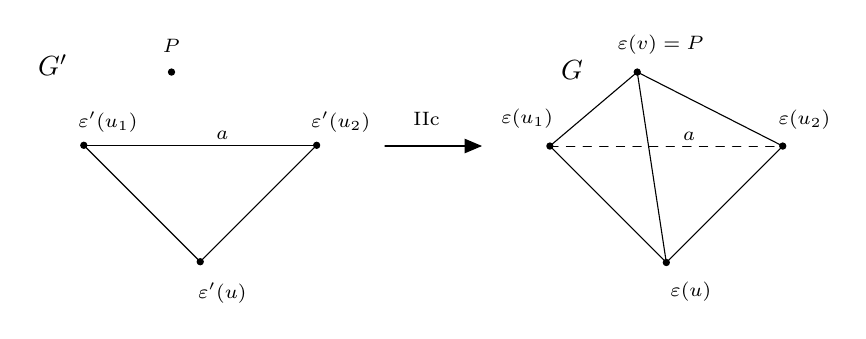
\begin{tikzpicture}[line cap=round,line join=round,>=triangle 45,x=1.0cm,y=1.0cm, scale=\textwidth/16.4cm]
%\clip(-1.238204075250744,-3.5306653610342322) rectangle (15.236984682261552,8.484974311111227);
\draw (0.04540876640913316,3.7210643089390185) node[anchor=north west] {$G'$};
\draw (9.030670131273066,3.6284327255634476) node[anchor=north west] {$G$};
\draw (5.,2.)-- (1.,2.);
\draw (1.,2.)-- (3.,0.);
\draw (3.,0.)-- (5.,2.);
\draw (9.006015420317214,1.9867669166606328)-- (11.006015420317214,-0.013233083339367235);
\draw (11.006015420317214,-0.013233083339367235)-- (13.006015420317217,1.9867669166606328);
\draw (10.50676,3.25791)-- (11.006015420317214,-0.013233083339367235);
\draw (10.50676,3.25791)-- (13.006015420317217,1.9867669166606328);
\draw (10.50676,3.25791)-- (9.006015420317214,1.9867669166606328);
\draw [->] (6.172322594794947,1.9875303914819094) -- (7.839691095555228,1.9875303914819094);
\draw [dash pattern=on 3pt off 3pt] (9.006015420317214,1.9867669166606328)-- (13.006015420317217,1.9867669166606328);
\begin{scriptsize}
\draw [fill=black] (10.50676,3.25791) circle (1.5pt);
\draw[color=black] (10.909767500655507,3.727680850608702) node {$\varepsilon(v)=P$};
\draw [fill=black] (11.006015420317214,-0.013233083339367235) circle (1.5pt);
\draw[color=black] (11.425857623232375,-0.5201389013281836) node {$\varepsilon(u)$};
\draw [fill=black] (9.006015420317214,1.9867669166606328) circle (1.5pt);
\draw[color=black] (8.615181352693646,2.450688308359763) node {$\varepsilon(u_1)$};
\draw [fill=black] (1.,2.) circle (1.5pt);
\draw[color=black] (1.4150325532477446,2.397755975002294) node {$\varepsilon'(u_1)$};
\draw [fill=black] (5.,2.) circle (1.5pt);
\draw[color=black] (5.411422733201952,2.397755975002294) node {$\varepsilon'(u_2)$};
\draw[color=black] (3.380144943059664,2.166177016563367) node {$a$};
\draw [fill=black] (3.,0.) circle (1.5pt);
\draw[color=black] (3.3801449430596646,-0.5333719846675509) node {$\varepsilon'(u)$};
\draw [fill=black] (13.006015420317217,1.9867669166606328) circle (1.5pt);
\draw[color=black] (13.377736932978223,2.437455225020396) node {$\varepsilon(u_2)$};
\draw[color=black] (6.886911160569152,2.4573048500294465) node {IIc};
\draw [fill=black] (2.5067616586988106,3.257906392061165) circle (1.5pt);
\draw[color=black] (2.5067616586988106,3.7144477672693346) node {$P$};
\draw[color=black] (11.399391463100228,2.152943933224) node {$a$};
\end{scriptsize}
\end{tikzpicture}
\caption{IIc with no vertex $w$}
\label{fig:IIc}
\end{figure}

IIb: We may assume that there are no vertices which can be constructed by Ia,b or IIa,c, i.e., all vertices of $G$ have degree at least four or can be constructed by IIb. Note that if $t$ denotes the number of vertices of degree three, then $t\geq 6$:
$$
2|V|-3=|E|=\frac{1}{2} \sum_{w\in V} \deg w\geq \frac{1}{2}\cdot 4(|V|-t)+\frac{1}{2}\cdot 3 t=2|V|-\frac{t}{2}\,.
$$

If there are three vertices in a triangle in $G$ such that all of them have degree three, then there is a nonrigid labelling and nontrivial bidistance by Theorem~\ref{thm:cutToTwoParts}.

Let there be a triangle induced by vertices $u,v, u_1\in V$ such that $\deg_G u =\deg_G v=3$ and $\deg_G u_1>3$. Let $w\in V\setminus \{v, u_1\}$ be the neighbour of $u$ and $u_2\in V\setminus \{u, u_1\}$ be the neighbour of $v$. We remark that the vertices $w$ and $u_1$ are nonadjacent, otherwise $u$ can be constructed by IIc. There are two possibilities: the easier case is  $wu_2\notin E$, since  a nonrigid labelling and nontrivial bidistance for $G$ are obtained by application of Theorem~\ref{thm:cutByVertices} with $V_c=\{u_1,u_2,w\}$. 

If $wu_2\in E$, then Lemma~\ref{lem:undoIIb} justifies that $G'$ can be indeed such that the vertex $v$ is constructed by linking to the vertices $u,u_1,u_2 \in V'$ such that $uu_1\in E',uu_2\notin E'$ and removing the edge $u_1u_2\in E'$, or the situation is symmetric by replacing $v$ by $u$ and $w$ by $u_2$, see Figure~\ref{fig:undoIIb}. Assume the former one. The degree of $u$ in $G'$ is two. Therefore, $G'$ can be obtained from $G''$ by adding the vertex $u$ by Henneberg move Ib. 

We show that the sum of connecting edges and \trcomps{} in $G''$ is at least two. Suppose in contrary that $G''$ is a single \trcomp{}. Since $u_1w\notin E_{G''}$, there must be some some other vertex $w'\in V_{G''}$ such that $u_1w',u_2w'\in E_{G''}$, i.e., $\deg_{G''} u_2 \geq 3$. Since $\deg_G u_1>3$, the degree of $u_1$ in $G''$ must be at least three. By Corollary~\ref{cor:atLeastTwoDegTwoInTrComp}, there are at least two vertices of degree two in $G''$. Hence, there is a vertex $v'\in V_{G''}\setminus\{u_1,u_2,w\}$ of degree two. But $\deg_{G''}v'=\deg_G v'$ which contradicts that all vertices of $G$ have degree at least three. 

By induction assumption, $G''$ is problematic or it has a nonrigid labelling and nontrivial bidistance. If the former holds, then $G$ is problematic by definition, otherwise we obtain a nonrigid labelling $\lambda$ of $G$ from the nonrigid labelling $\lambda''$ of $G''$ in the following way: let $\varepsilon''$ be an embedding of $G''$ compatible with $\lambda''$ such that there are infinitely many embeddings of $G''$ compatible with $\lambda''$ in the neighbourhood of $\varepsilon''$. We define an embedding $\varepsilon$ of $G$ such that $\varepsilon|_{V_{G''}}=\varepsilon''$, $\varepsilon(u)$ satisfies $||\varepsilon(u)-\varepsilon(u_1)||^2=\lambda''(u_1u_2)=:a^2$ and $||\varepsilon(u)-\varepsilon(w)||^2=\lambda''(wu_2)=:b^2$, and $\varepsilon(v)$ satisfies $||\varepsilon(u)-\varepsilon(v)|| =||\varepsilon(v)-\varepsilon(u_2)||$. Now we obtain $\lambda$ be measuring distances in $\varepsilon$, i.e., $\lambda(u'v')=||\varepsilon(u')-\varepsilon(v')||^2$ for all $u'v'\in E_G$. The construction of $\lambda$ guaranties that there is an embedding of $G$ compatible with $\lambda$ corresponding to every embedding in the neighbourhood of $\varepsilon'$.
%$$
%\lambda(e)=\begin{cases}
%\lambda''(e) \text{ if } e\in E_{G''}\setminus u_1u_2\\
%\lambda''(u_2w) \text{ if } e=uw\\
%\lambda''(u_1u_2) \text{ if } e=uu_1\\
%c \text{ if } e\in\{uv,u_2v\}\\
%d \text{ if } e=u_1v\,,
%\end{cases}
%$$
%where $c=||\varepsilon(u_2)-P||^2$ and $d=||\varepsilon(u_1)-P||^2$ for some point $P\in\RR^2$ and an embedding $\varepsilon$ of $G''$ compatible with $\lambda''$.
\begin{figure}[htb!]
\centering
\begin{tikzpicture}[line cap=round,line join=round,>=triangle 45,x=2.1cm,y=2.1cm]%, scale=\textwidth/4.0cm]
\draw [->] (6.275266360419553,4.) -- (6.775266360419553,4.);
\draw (7.867239418548063,2.983115429032273)-- (9.358688293471314,2.990059134751416);
\draw (9.358688293471314,2.990059134751416)-- (8.496658480471117,4.082983993393495);
\draw (8.496658480471117,4.082983993393495)-- (7.117654339044025,4.272530090862931);
\draw (7.117654339044025,4.272530090862931)-- (7.867239418548063,2.983115429032273);
\draw (7.117654339044025,4.272530090862931)-- (8.94770248650687,4.871153836655923);
\draw (8.94770248650687,4.871153836655923)-- (8.496658480471117,4.082983993393495);
\draw (7.070390124337253,5.301368950823323) node[anchor=north west] {$G$};
\draw (4.297012237032155,2.9209111346261687)-- (5.788461111955406,2.9278548403453115);
\draw (3.8545153496234357,5.301368950823323) node[anchor=north west] {$G''$};
\draw (5.377475304990962,4.808949542249815)-- (5.788461111955406,2.9278548403453115);
\draw [dash pattern=on 1pt off 1pt] (8.94770248650687,4.871153836655923)-- (9.358688293471314,2.990059134751416);
\begin{scriptsize}
\draw [fill=black] (8.94770248650687,4.871153836655923) circle (1.5pt);
\draw[color=black] (9.355975853484337,4.937201946718099) node {$\varepsilon(u_1)$};
\draw [fill=black] (7.867239418548063,2.983115429032273) circle (1.5pt);
\draw[color=black] (7.821134409723406,2.7662063453215713) node {$\varepsilon(w)$};
\draw[color=black] (6.571761457177793,4.194861515272835) node {Ib, IIb};
\draw [fill=black] (9.358688293471314,2.990059134751416) circle (1.5pt);
\draw[color=black] (9.779232377950722,2.8418410307895794) node {$\varepsilon(u_2)$};
\draw[color=black] (8.588686402991337,3.1135656415450157) node {$b$};
\draw [fill=black] (8.496658480471117,4.082983993393495) circle (1.5pt);
\draw[color=black] (8.493442724994587,3.830694511167611) node {$\varepsilon(v)$};
\draw[color=black] (8.913635422039075,3.6962328481133744) node {$c$};
\draw [fill=black] (7.117654339044025,4.272530090862931) circle (1.5pt);
\draw[color=black] (7.18804407950971,4.446977133499528) node {$\varepsilon(u)$};
\draw[color=black] (8.006019196422981,4.228476931036393) node {$c$};
\draw[color=black] (7.3337108811517995,3.561771185059138) node {$b$};
\draw[color=black] (8.017224335010834,4.710297890314075) node {$a$};
\draw [fill=black] (5.377475304990962,4.808949542249815) circle (1.5pt);
\draw[color=black] (5.913459565141429,4.77472743719423) node {$\varepsilon''(u_1)$};
\draw [fill=black] (4.297012237032155,2.9209111346261687) circle (1.5pt);
\draw[color=black] (4.285913185255777,2.7045780830883794) node {$\varepsilon''(w)$};
\draw [fill=black] (5.788461111955406,2.9278548403453115) circle (1.5pt);
\draw[color=black] (6.294434277128431,2.7465973527928287) node {$\varepsilon''(u_2))$};
\draw[color=black] (5.025452332054077,3.0575399486057506) node {$b$};
\draw[color=black] (5.753786340264523,3.875515065519023) node {$a$};
\draw[color=black] (9.300212703320005,3.9147330505765088) node {$a$};
\end{scriptsize}
\end{tikzpicture}
\caption{Embedding $\varepsilon$}
\label{fig:IIc}
\end{figure}
The existence of nontrivial bidistance follows by Theorem~\ref{thm:nonrigidImplieBidistance} or we can construct it explicitly: the bidistance of the edge $uw$ set the same as bidistance of $wu_2$ in $G''$ and the bidistance of all other new edges set the bidistance of $u_1u_2$ in $G''$.

The remaining graphs are such that all vertices have degree at least three and if $v$ has degree three, then precisely two neighbours $u,u_1$ of $v$ are adjacent and have degree at least four. Let $u_2$ be the third neighbour of $v$. Assume that $u_1$ is not a connecting vertex. We show that we can revert the last Henneberg move by removing $v$ and adding the edge $u_1u_2$. According to Theorem~6.4 in (Laman), this is possible if there is no subgraph $M$ of $G\setminus v$ such that $u_1,u_2\in V_M$ and $|E_M|=2|V_M|-3$. Suppose in contrary that there is such subgraph $M$. Let $T$ be the \trcomp{} of $u_1, u$ and $v$ in $G$. Since $u_1$ is not connecting vertex, $T'=T\setminus v$ is a \trcomp{} in $G\setminus v$. Since $M$ is connected and $u_2\in V_M$, there must be at least two vertices in $V_{T'}\cap V_M$. By Lemma~6.2 in  (Laman), the subgraph $H$ of $G$ induced by $V_{T'}\cup V_M$ satisfies $|E_H|=2|V_H|-3$. But then there are too many edges in the subgraph induced by $V_H\cup\{v\}$, namely there are edges $u_1v, uv$ and $u_2$ besides the edges of $H$, while there is only one more vertex. Therefore, there is a graph $G'$ such that $G$ is constructed from $G'$ by adding the vertex $v$ and removing the edge $u_1u_2$. If $G'$ is problematic, then $G$ is problematic by definition. If $G'$ has a nonrigid labelling $\lambda'$, then a nonrigid labelling $\lambda$ of $G$ is given as follows: let $\varepsilon'$ be an embedding of $G'$ compatible with $\lambda'$ and let $\varepsilon$ be an embedding of $G$ such that 
$$
\varepsilon(w)=\begin{cases}
\varepsilon'(u_1) \text{ if } w=v\\
\varepsilon'(P) \text{ for some }P\in \RR^2 \text{ if } w=u_1\\
\varepsilon'(w) \text{ otherwise.}
\end{cases}
$$
Now $\lambda(ww')=||\varepsilon(v)-\varepsilon(w')||^2$ for all $ww'\in E$. Using nontrivial bidistance $\delta'$ of $G'$, the nontrivial bidistance $\delta$ of $G$ is defined by $\delta(uv)=\delta(u_1v)=\delta'(uu_1)$, $\delta(u_2v)=\delta'(u_1u_2)$ and $\delta(e)=\delta'(e)$ otherwise. We proceed analogically if $u$ is not connecting vertices.

To conclude, we proved the claim for all graphs except for such that all vertices have degree at least three and if some vertex has degree three, then precisely two its neighbours are adjacent, both have degree at least four and both are connecting vertices. But those are basic problematic.
\end{proof}

\end{document}